\documentclass[../momento_1.tex]{subfiles}

Esta fase tinha como propósito a construção da \textit{unpredictable MIB} que será utilizada para o agente SNMP guardar os parâmetros de configuração e os números aleatórios. Foram utilizados dois programas externos: o \textit{MIB Designer} e o \textit{AgenPro}.\par

O \textit{MIB Designer} serve para construir e editar a MIB através de uma interface gráfica facilitando assim a sua conceção, evitando erros de sintaxe e semântica. O \textit{AgenPro} foi utilizado para gerar o código Java da \textit{unpredictable MIB} através do ficheiro criado pelo \textit{MIB Designer}.\par

A MIB possui dois grupos: \textit{unpredictableParam} e \textit{unpredictableTable}. O grupo \textit{unpredictableParam} possui os objetos escalares(R, N e D) que representem os parâmetros de funcionamento e ainda um objeto escalar especial (do tipo \textit{string} e apenas com permissões de escrita) que servirá para verificar autorizações para a operação \textit{reset} do agente como podemos ver na Figura \ref{fig:unpredictableParam}.\\

\begin{figure}[H]
\centering
\captionsetup{justification=centering,margin=4cm}
\centerline{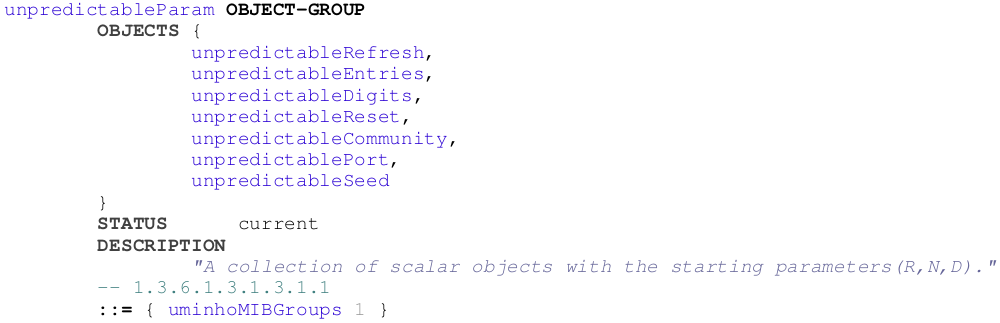
\includegraphics[scale=0.4]{../imagens/unpredictableParam.png}}
\caption{Grupo \textit{unpredictableParam}.}\\[7cm]
\label{fig:unpredictableParam}
\end{figure}


O grupo \textit{unpredictableTable} contém a tabela de N números aleatórios com apenas duas colunas, uma para o índice de entrada (chave da tabela) e outra para o número aleatório (sequência de D dígitos hexadecimais), como está exemplificado na Figura \ref{fig:unpredictableTable}.\\

\begin{figure}[H]
\centering
\captionsetup{justification=centering,margin=4cm}
\centerline{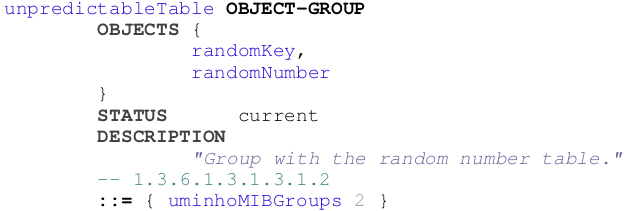
\includegraphics[scale=0.5]{../imagens/unpredictableTable.png}}
\caption{Grupo \textit{unpredictableTable}.}
\label{fig:unpredictableTable}
\end{figure}

Com a \textit{unpredictable MIB} definida obtém-se o código Java exemplificado no Exemplo \ref{fig:unpredictableJAVA}.\\

{\setstretch{1.1}
\begin{lstlisting}[caption={Exemplo código JAVA \textit{unpredictable} MIB},label={fig:unpredictableJAVA},language=JAVA]
	 public static final OID oidUminhoGrMib =
    new OID(new int[] { 1,3,6,1,3,1 });

  // Identities
  // Scalars
  public static final OID oidUnpredictableRefresh = 
    new OID(new int[] { 1,3,6,1,3,1,1,1,0 });
  public static final OID oidUnpredictableEntries = 
    new OID(new int[] { 1,3,6,1,3,1,1,2,0 });
  public static final OID oidUnpredictableDigits = 
    new OID(new int[] { 1,3,6,1,3,1,1,3,0 });
  public static final OID oidUnpredictableReset = 
    new OID(new int[] { 1,3,6,1,3,1,1,4,0 });
  public static final OID oidUnpredictableCommunity = 
    new OID(new int[] { 1,3,6,1,3,1,1,6,0 });
  public static final OID oidUnpredictablePort = 
    new OID(new int[] { 1,3,6,1,3,1,1,7,0 });
  public static final OID oidUnpredictableSeed = 
    new OID(new int[] { 1,3,6,1,3,1,1,8,0 });
  // Tables
  
  // Notifications
  
  // Enumerations
  
  // TextualConventions
  
  private static final String TC_MODULE_SNMPV2_TC = "SNMPv2-TC";
  private static final String TC_DISPLAYSTRING = "DisplayString";

  // Scalars
  private MOScalar<Integer32> unpredictableRefresh;
  private MOScalar<Integer32> unpredictableEntries;
  private MOScalar<Integer32> unpredictableDigits;
  private MOScalar<OctetString> unpredictableReset;
  private MOScalar<OctetString> unpredictableCommunity;
  private MOScalar<Integer32> unpredictablePort;
  private MOScalar<OctetString> unpredictableSeed;

  // Tables
  public static final OID oidRandomEntry = 
    new OID(new int[] { 1,3,6,1,3,1,1,5,1 });

  // Index OID definitions
  public static final OID oidRandomKey =
    new OID(new int[] { 1,3,6,1,3,1,1,5,1,1 });
  public static final OID oidRandomNumber =
    new OID(new int[] { 1,3,6,1,3,1,1,5,1,2 });
\end{lstlisting}}
\clearpage
